\chapter{Marco teórico}

\section{Inteligencia artificial, aprendizaje automático y aprendizaje profundo}
\todo{Reformar esta sección para incluir la IA generativa y establecer las relaciones con el resto de conceptos}
Comencemos por definir las diferentes disciplinas que intervienen en el estudio y desarrollo de sistemas de inteligencia artificial. A menudo se encuentran términos como \textit{inteligencia artificial} (\textit{Artificial Intelligence}), \textit{aprendizaje automático} (\textit{Machine Learning}) y \textit{aprendizaje profundo} (\textit{Deep Learning}) usados de forma intercambiable. Sin embargo, cada uno tiene un significado específico, y es crucial diferenciarlos para comprender el estado actual de la investigación en el área. Estos conceptos se organizan jerárquicamente \citep{torresivinalsPythonDeepLearning2020}, donde la inteligencia artificial es el término más general, que abarca el \textit{aprendizaje automático}, y este último incluye al \textit{aprendizaje profundo} (ver Figura \ref{fig:ai_ml_dl}).

\begin{figure}[h]
    \caption{Relación AI, ML y DL}
    \centering
    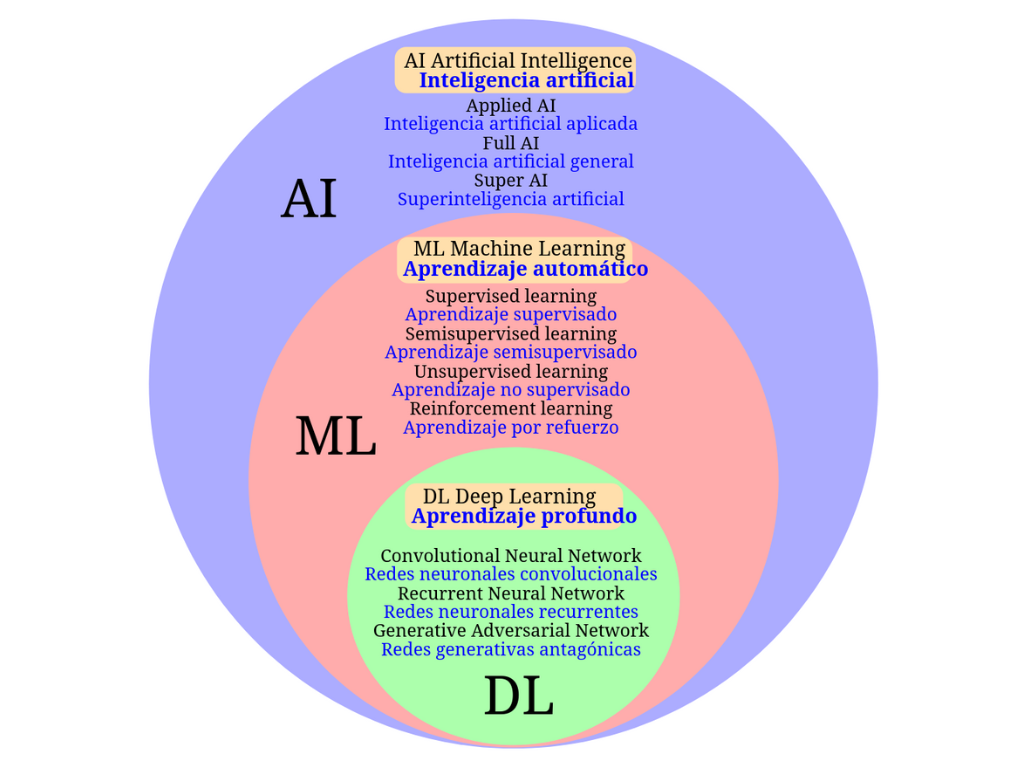
\includegraphics[width=0.8\textwidth]{./figuras/AI_ML_DL.png}
    \source{Jzh2074 \protect\citeyear{jzh2074}, Wikimedia Commons; Wang et al. \protect\citeyear{wang2021promising}.}
    \label{fig:ai_ml_dl}
\end{figure}

% He añadido una imagen de relación AI, ML, DL y AI generativa. Sería interesante modificar lo anterior para hablar también de la IA generativa, que al fin y al cabo es la que nos interesa. La imagen la he sacado de aquí: https://medium.com/@kitkat73275/introduction-to-generative-ai-833c9c467dfa (añadirla a bibliografía y citarla)


La inteligencia artificial es el campo de estudio más antiguo entre los tres, y no se limita únicamente al ámbito computacional. En su sentido más amplio, la inteligencia artificial ha sido abordada por la filosofía. Los racionalismos y estructuralismos, fundamentales en los sistemas de pensamiento occidentales, forman la base conceptual de la inteligencia artificial. Sin embargo, no es hasta el siglo XX cuando se empieza a considerar la posibilidad matemática de un sistema que genere inteligencia. En 1950, Alan Turing publicó su artículo \textit{Computing Machinery and Intelligence} \citep{alan1950a}, en el que propuso un test para determinar si una máquina puede pensar. Este test, conocido como \textit{Test de Turing}, consiste en la interacción de un humano con una entidad artificial usando solo un terminal de texto como interfaz. La máquina aprueba el test si el humano no puede discernir si está interactuando con una entidad artificial o humana. A pesar de sus limitaciones y su enfoque antropocéntrico sobre la inteligencia, este test sigue siendo una referencia común para evaluar sistemas modernos de IA.

No obstante, el concepto de inteligencia artificial trasciende la mera imitación humana, aunque no lo descarta. Si consideramos la \textit{racionalidad} como un conjunto de estructuras lógicas que incluyen el pensamiento y la racionalidad humanos, la inteligencia artificial no necesita limitar su objetivo a superar el test de Turing. Las definiciones de inteligencia artificial a lo largo del tiempo han variado dependiendo de si se enfocan en imitar el pensamiento o acción \textit{humanos} o el pensamiento y acción \textit{racional} \citep{RussellStuartJ2021AI:A}.

Debemos a matemáticos como Alan Turing y Curt Gödel los fundamentos matemáticos de los procesos de pensamiento, considerados sistemas computacionales capaces de generar \textit{outputs} racionales a partir de \textit{inputs} arbitrarios. La idea de que el cerebro humano es una de las posibles \textit{máquinas de Turing} \citep{penroseNuevaMenteEmperador2015} ha sido un estímulo para la investigación en IA computacional. Además, investigaciones en \textit{procesamiento del lenguaje natural}, en las que destaca el concepto de \textit{entropía} de Shannon \citep{shannon1951prediction} y que han acompañado el desarrollo de lenguajes de programación, son fundamentales para los sistemas actuales de IA.


\section{Machine Learning}

El \textit{Machine Learning}, o \textit{aprendizaje automático}, es una subdisciplina de la inteligencia artificial que investiga algoritmos y modelos matemáticos que habilitan a un sistema computacional a aprender a partir de datos sin ser explícitamente programado. Estos sistemas identifican patrones y toman decisiones con poca o sin intervención humana. En el \textit{Machine Learning}, el modelo se autoconfigura basándose en los datos. Las únicas intervenciones humanas son el diseño de la arquitectura y la provisión de los datos de entrenamiento, aunque incluso estas tareas podrían delegarse a otro sistema de \textit{Machine Learning} en determinadas circunstancias.

Aunque el \textit{Machine Learning} ha sido una área de interés desde los inicios de la computación, es esencial reconocer que es solo una faceta de la inteligencia artificial. No todos los sistemas inteligentes son sistemas de \textit{Machine Learning}. Por ejemplo, el \textit{Deep Blue} de IBM, que venció al campeón mundial de ajedrez Garry Kasparov en 1997, no se basaba en \textit{Machine Learning} \citep{campbellDeepBlue2002}. En lugar de ello, \textit{Deep Blue} utilizaba una vasta base de datos de jugadas de ajedrez y algoritmos de búsqueda para decidir el mejor movimiento en cada situación. Otros sistemas, como los \emph{sistemas expertos}, utilizan reglas predefinidas para tomar decisiones y se aplican en áreas como medicina, ingeniería y gestión empresarial.

En términos generales, el objetivo del \textit{Machine Learning} es encontrar una función matemática que describa un conjunto de datos de entrenamiento y que, posteriormente, pueda prever datos desconocidos con precisión. Esta capacidad predictiva se conoce como \textit{inferencia}. El proceso busca que la función determinada durante el entrenamiento aproxime la función real que describe los datos, permitiendo al sistema generalizar de forma análoga al cerebro humano.

Se utiliza el término \textit{modelo} para referirse al sistema una vez que ha sido entrenado y posee capacidad predictiva. Dependiendo de su aplicación, un modelo puede ser empleado para predecir datos desconocidos o clasificarlos. Si produce un valor numérico, se habla de \textit{regresión}; si categoriza datos, de \textit{clasificación}. La clasificación puede ser binaria o multiclase, y la regresión unidimensional o multidimensional.

El aprendizaje en \textit{Machine Learning} se produce a través de un proceso de entrenamiento. Según la naturaleza de los datos y el método de validación, existen tres tipos principales de aprendizaje automático \citep[p. ~38]{torresivinalsPythonDeepLearning2020}:

\begin{itemize}
    \item \textbf{Aprendizaje supervisado:} Aquí, los datos se etiquetan con la respuesta esperada, como imágenes de animales etiquetadas como \textit{gato} o \textit{perro}. Tras el entrenamiento, se espera que el sistema identifique imágenes no etiquetadas correctamente.
    
    \item \textbf{Aprendizaje no supervisado:} En este caso, los datos no están etiquetados. El sistema busca patrones y agrupa datos en categorías por sí mismo.
    
    \item \textbf{Aprendizaje por refuerzo:} El sistema aprende interactuando con un entorno. No recibe etiquetas explícitas, sino recompensas por decisiones correctas y penalizaciones por errores.
\end{itemize}


\section{Deep Learning}

qué es el Deep Learning, y por qué ha evolucionado tanto en los últimos años, factores: poder computacional, cantidad de datos disponibles, democratización de la computación, mejoras en las arquitecturas y modelos de Deep Learning.

A partir de ahí se explican detalles desde las redes neuronales hasta Transformer, que es el estado del arte actual de deep learning, incluyendo los modelos de lenguaje que nos atañen.


\subsection{Tipos de redes neuronales}
\subsection{Arquitecturas de redes neuronales}
\subsection{Datos y entrenamiento de modelos de \textit{Deep Learning}}

\subsection{La arquitectura Transformer}

En la Figura \ref{fig:transformer_architecture} se puede ver un esquema de la arquitectura \textit{Transformer}.

\begin{figure}[h]
    \caption[Aquitectura de Transformer]{Aquitectura de Transformer}
    \centering
    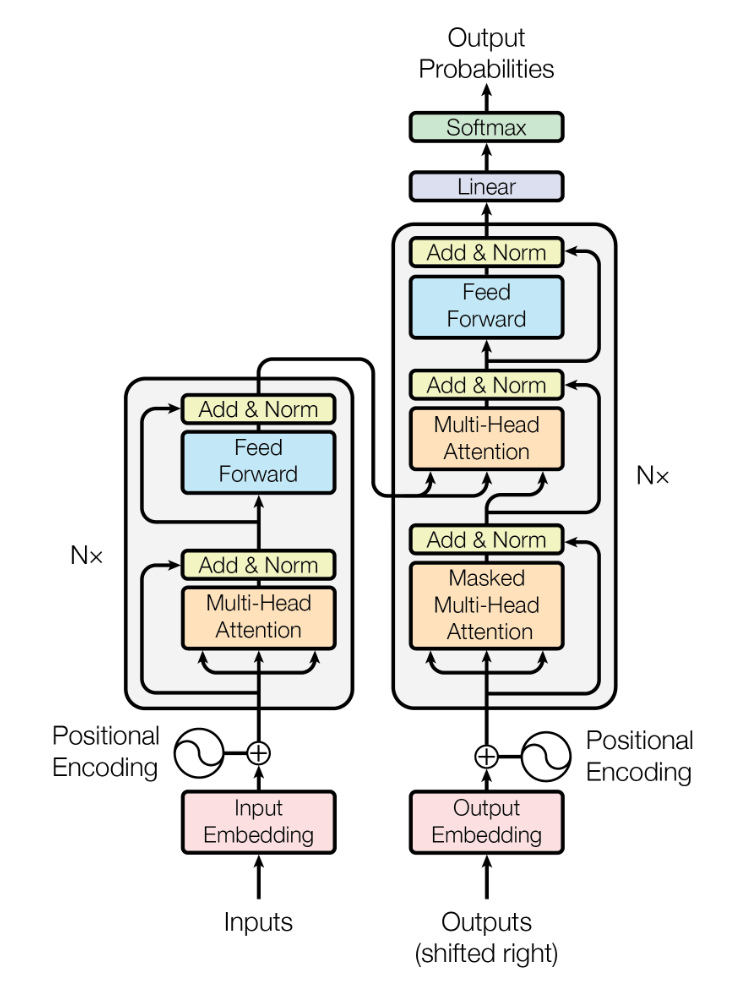
\includegraphics[width=0.4\textwidth]{./figuras/Transformer_architecture.png}
    \source{\cite{vaswaniAttentionAllYou2017}}
    \label{fig:transformer_architecture}
\end{figure}

\section{Modelos de lenguaje}

Un \textit{modelo de lenguaje} es un modelo estadístico que asigna una probabilidad a una secuencia de palabras dada como entrada. Esencialmente, es una función matemática diseñada para simular la forma en que se escribe en lenguaje natural. Una analogía común para entender el funcionamiento de un \textit{modelo de lenguaje} es la función predictiva de un teclado. Mientras escribimos en nuestro dispositivo móvil, el teclado nos sugiere palabras que probablemente seguirán a las ingresadas. Esta capacidad de predicción es el fundamento de los \textit{modelos de lenguaje}, incluyendo chatbots avanzados.

Desde una perspectiva técnica, un \textit{modelo de lenguaje} devuelve como salida la distribución de probabilidad del siguiente \textit{token}, dada una secuencia de \textit{tokens} como entrada \citep{GenerationLLMs}. Un \textit{token} es la unidad mínima de información que el modelo procesa y, generalmente, equivale a una palabra\footnote{Aunque un token suele ser una palabra, también puede ser un signo de puntuación, número o cualquier otra unidad mínima de información.}. La Figura \ref{fig:llm_generation} ilustra un \textit{modelo de lenguaje} que recibe una secuencia de palabras y devuelve la distribución de probabilidad del siguiente \textit{token} después de haber sido entrenado con textos en inglés.

\begin{figure}[h]
    \caption[Inferencia de \textit{token} de un LLM]{Inferencia de \textit{token} de un LLM}
    \centering
    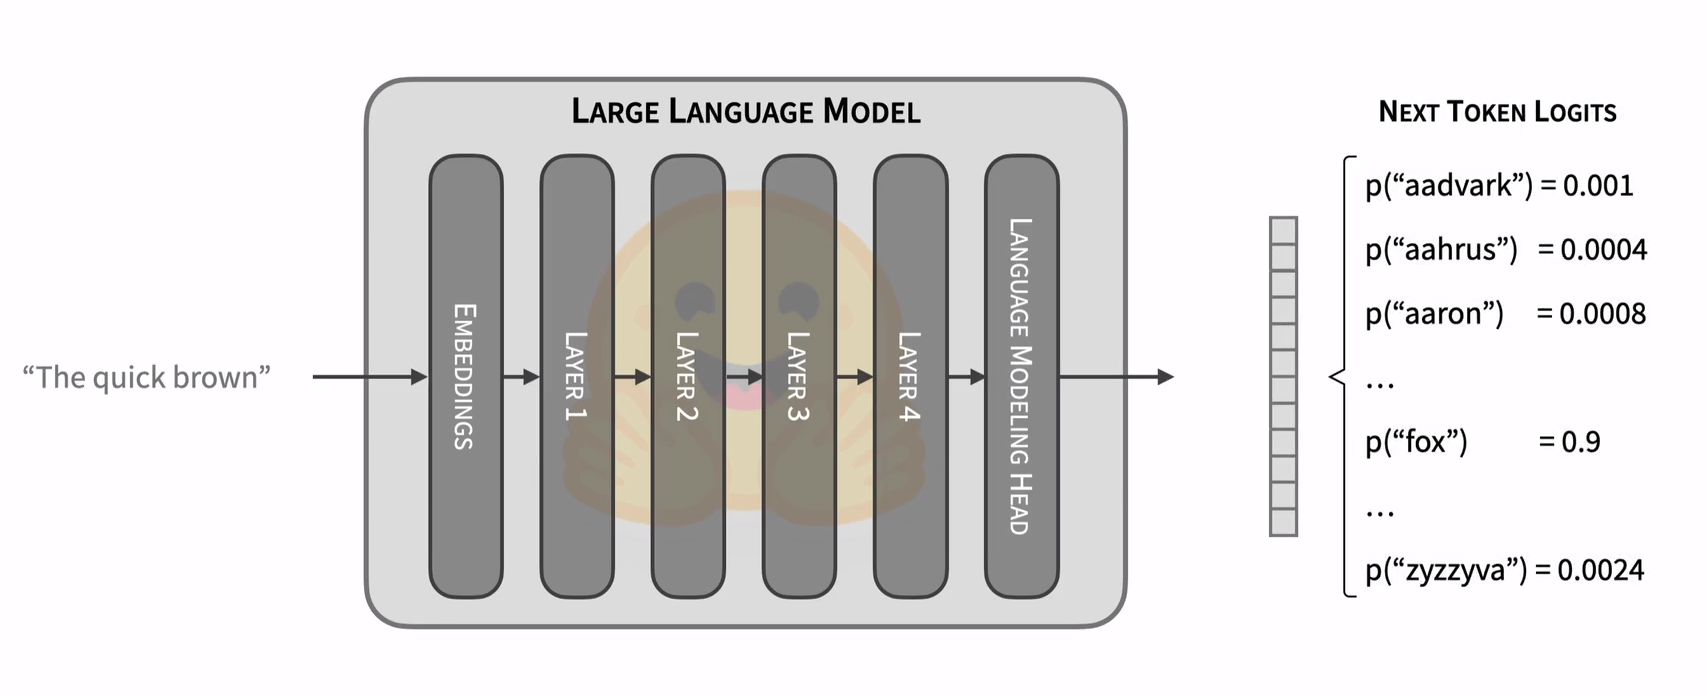
\includegraphics[width=0.9\textwidth]{./figuras/LLM_predice_token.png}
    \source{\cite{GenerationLLMs}}
    \label{fig:llm_generation}
\end{figure}

Los \textit{modelos de lenguaje} no se asocian exclusivamente a una arquitectura de \textit{Machine Learning}. Pueden implementarse mediante diferentes tipos de redes neuronales, como las redes neuronales recurrentes, convolucionales o Transformer. No obstante, el hito que ha propulsado avances significativos en \textit{Machine Learning} ha sido la arquitectura \textit{Transformer} \citep{vaswaniAttentionAllYou2017}. 

\subsection{Grandes modelos de lenguaje}

Un \textit{gran modelo de lenguaje} (LLM) posee un número de parámetros del orden del billón. El primer LLM fue \textit{GPT-2}, creado y entrenado por OpenAI en 2019 \citep{radfordLanguageModelsAre2019a}. \textit{GPT-2} se entrenó con 40 GB de texto de Internet y alcanzó 1.5 billones de parámetros. Su capacidad para predecir la siguiente palabra en una secuencia sorprendió a la comunidad científica debido a la calidad de los textos generados. Sin embargo, OpenAI publicó una versión reducida de 117 millones de parámetros debido a preocupaciones sobre su eventual uso irresponsable. La Figura \ref{fig:gpt2_text_generation} muestra ejemplos de textos generados por este modelo.

\begin{figure}[h]
    \caption{Generación de textos por \textit{GPT-2}}
    \centering
    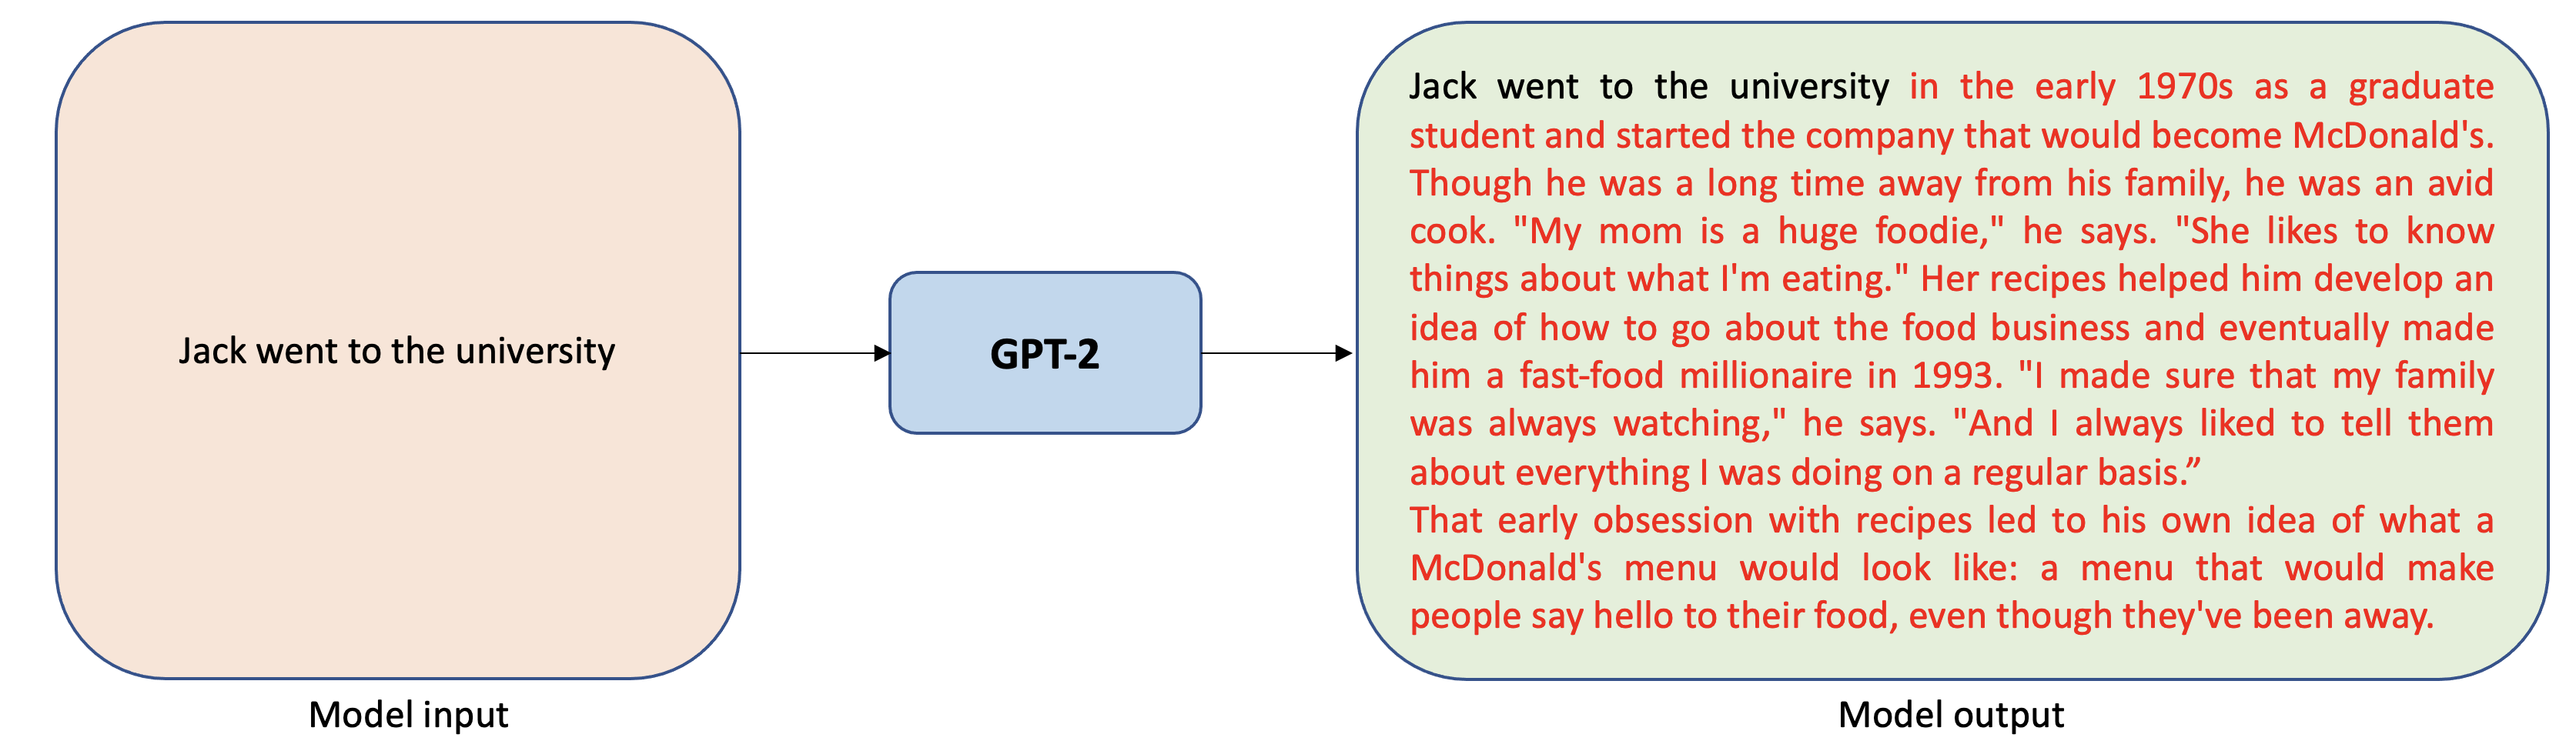
\includegraphics[width=0.9\textwidth]{./figuras/GPT2_text_generation.png}
    \source{\cite{RunTextGeneration2022}}
    \label{fig:gpt2_text_generation}
\end{figure}

Los \textit{grandes modelos de lenguaje} emplean la arquitectura \textit{Transformer}, introducida por \citeauthor{vaswaniAttentionAllYou2017} en 2017, que ha proporcionado una eficiencia computacional sin parangón.

\begin{figure}[h]
    \caption{Gráfico comparativo de tamaños de LLM}
    \centering
    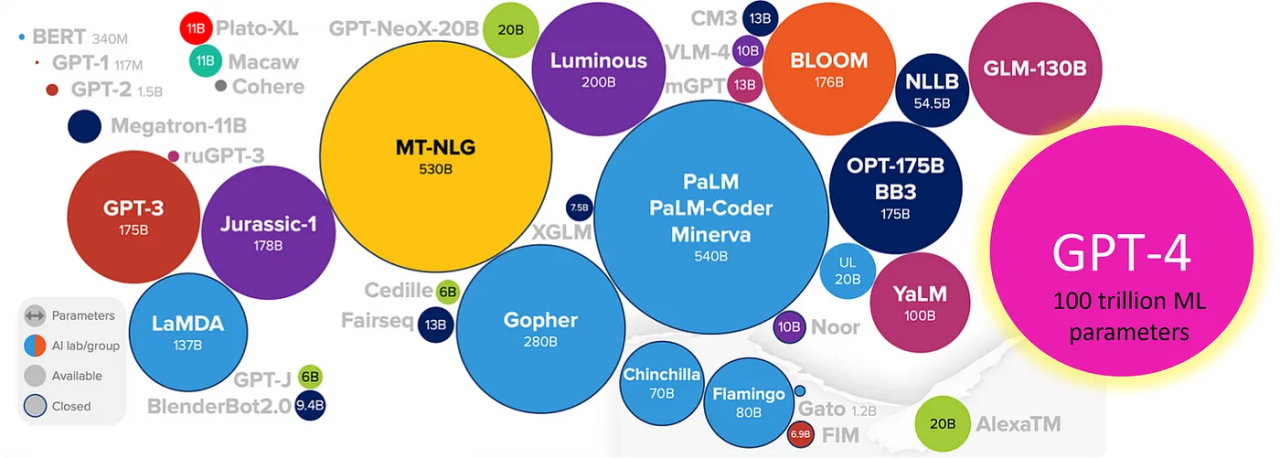
\includegraphics[width=0.9\textwidth]{./figuras/LLMs_sizes.png}
    \source{\cite{ChallengesAssociatedBuilding}}
    \label{fig:llm_sizes}
\end{figure}

\subsection{Modelos preentrenados}
\subsection{Ajuste fino de los modelos}
Bibliografía: \cite{chamandFinetuneYourClassifier2022}

\subsection{Hiperparámetros fijos del modelo}
Aquí hablaré de los hiperparámetros que definen la arquitectura del modelo que no se pueden modificar, como el número de capas, el número de cabezas de atención, etc., y que son fijos en el modelo. Especial atención se pondrá en el número de parámetros del modelo, que es el que determina el tamaño del modelo y su capacidad de generar textos, así como en la ventana de contexto, que es el número de tokens que el modelo tiene en cuenta para generar el siguiente token.

Precisamente el número de parámetros y la ventana de contexto son los hiperparámetros más importantes y críticos en términos computacionales y de efectividad. Cuanto más grande sea el modelo, más parámetros tendrá y más capacidad de generar textos tendrá. Sin embargo, también será más lento en la inferencia. Por otro lado, cuanto mayor sea la ventana de contexto, más tokens tendrá en cuenta el modelo para generar el siguiente token, y más coherentes serán los textos generados. Sin embargo, también será más lento en la inferencia.

\subsection{Hiperparámetros controlables por el usuario}
Hablar de la temperatura, top\_p, top\_k, ventana de contexto, número de tokens, etc. 

Se habla de la temperatura y su impacto en la generación de textos en \cite{holtzmanCuriousCaseNeural2020} y \cite{chamandFinetuneYourClassifier2022}

\cite{holtzmanCuriousCaseNeural2020} habla de la importancia de top\_p, en lo que denomina \textit{top\_k nucleus sampling}. Aunque es antiguo el paper, echar un ojo porque aclara bastante los conceptos.

Seguimos las explicaciones de \cite{rothmanTransformersNaturalLanguage2021}

Existen estudios centrados en la optimización de los hiperparámetros (los ya citados más arriba y \cite{wangCostEffectiveHyperparameterOptimization2023} y \cite{wangHyperparameterOptimizationAlgorithm2022})


\subsection{Habilidades emergentes de los modelos de lenguaje}
\subsection{Prompting engineering}
En esta sección se abordará la disciplina del \textit{prompting engineering} y se ofrecerá una visión general de sus enfoques \citep{LLMPromptingGuide}\dots


\section{SuperCollider}

